\subsection{Investigation and spike}
  After initiation the project is investigated and then \textit{spiked}. In this case investigation/research for the most part has been done,
  as we knew the system was feasible due to following the same design as our catalogue pipeline. However it was determined that a spike of the 
  proposed algorithm would be done.

  \begin{figure}[H]
    \centering
    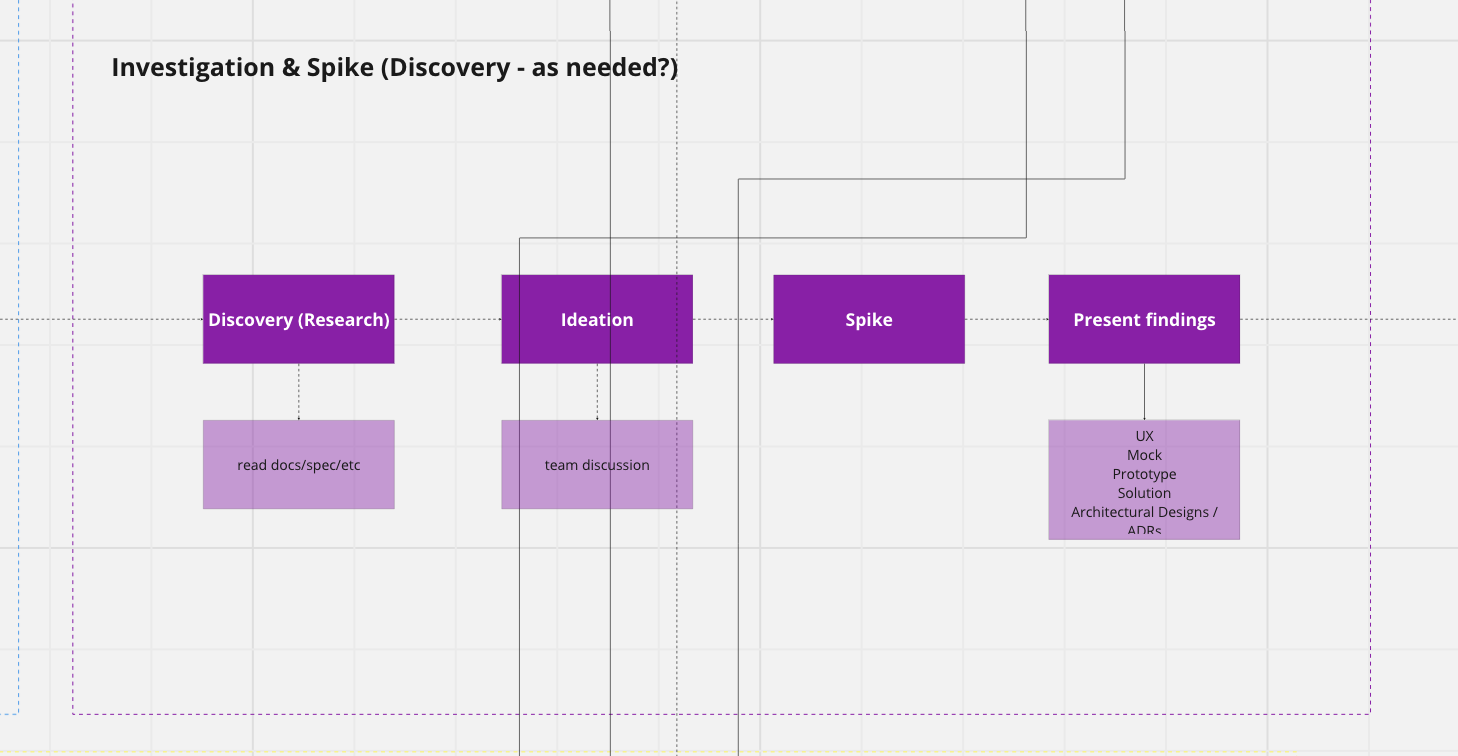
\includegraphics[width=8cm]{assets/workflow/investigation.png}
    \caption{Investigation stage of our ways of working.}
    \label{fig:workflowInvestigation}
  \end{figure}

  A spike is often used when there are unknowns about a  project (Visual Paradigm, 2024). A study done by 
  Hashimi and Gravell (2020) found that a majority of people in industry saw spikes as an effective tool and helped in managing risks. In another
  study they also stated that one of key purposes of a spike was to help guide story/ticket estimations (Hashimi, Gravell, 2019). 

  In the first paper it was also hypothesised that technical debt can also be lowered through the use of spikes, with technical debt be defined as:
  \begin{quote}
    \textit{'the idea that developers sometimes accept
    compromises in a system in one dimension (e.g., modularity) to meet an
    urgent demand in some other dimension (e.g., a deadline)' (Kruchten et al, 2012)}
  \end{quote}

  Spikes were used by Glas and Hedén (2021) to help bring down technical debt in their study. However when thought about simply, 
  a spike could be seen as a tool to spot the technical debt before it touches live systems. Due to a prototype being made flaws can be spotted 
  early and ironed out before the \textit{'real'} development work begins.

  For the project a spike was carried out to test the algorithms outlined in \hyperref[sec:AppendixC]{\textbf{Appendix C}} to test the 
  throughput of the system and see if it could handle the incoming requests. We used the technical spike template recommended by Microsoft (2021), to 
  document findings and outline the spikes objectives. Hashimi, Abduldaem and Gravell (2022) found that  \textit{'timeboxing, objectives,
  documentation, and clear communication'} were the key factors that lead to a successful spike.

  There was no time limit set, which did lead to scope creep (Martins, 2023) and more time being spent than was necessary. It's important to remember that a 
  spike is not meant to be the final product, however scope creep lead to the spike being almost a fully working system, albeit unrefined and with issues. 
  This is something as a team we have now changed in our process and will always time-box spikes in the future to prevent this.

  Despite this the other key factors were well adhered to. Objectives and documentation of the spike were put into a spike document
  and we had communication with a more senior member of the team at all times as well as daily stand ups to communicate issues/progress on the spike. 
  \footnote{P4 - This section demonstrates self-direction and originality to improve a design created by a more senior developer.}
  \footnote{SE-S02 - This section also demonstrates the evaluation of the design and recommends both current and future improvements that can be made.
  In this case cloud technologies such as lambda and dynamoDB are recommended in the spikes output.}
  The full spike document can be seen in \hyperref[sec:AppendixE]{\textbf{Appendix E}}, below are the key findings.

  \begin{enumerate}
    \item A garbage collector should be used to clean up data that is no longer referenced by a schedule. This will help lower the amount of redis sets/gets
    and has no negative affect on partners.
    \item When a catalogue item (episode/series/brand) updates it will also need to update it's associated schedules, for titling and descriptions. This in 
    itself is not a problem, however if the number of schedules referenced is large it can significantly slow the system down. Parallelisation should be 
    looked into, at least at the schedule level to help ease this. Full parallelisation would require a new design to support parallelised editing of the 
    broadcast list held in episodes (this discussed in the \hyperref[sec:storageSolutions]{\textbf{Research}} section).
    \item Redis duplication is complex and is only needed so that episodes can reference a list of schedules that they are in. Might be worth using 
    DynamoDB here as this will also help with parallelisation (This is explored in the \hyperref[sec:future]{\textbf{Future Work}} section).
    \item Additional filtering from the catalogue pipeline could be added to only send updates for items that are referenced by a schedule. This would 
    stop lambda being ran that essentially do nothing, this is also discussed in \hyperref[sec:future]{\textbf{Future Work}}.
  \end{enumerate}

  It was determined by the team that, for now, the system should be single-threaded and stick to the original design due to time constraints.
  Parallelisation could be looked into in the future when we had some time. However it was agreed for a garbage collector to be used and 
  when a batch of schedule updates is is triggered by a catalogue update that some form of concurrency would be required. This can be done with schedule
  objects due to the single threaded nature of the current system. As the schedule updates are being done because of a catalogue update the only 
  fields that can change are the titles and descriptions. These do not affect or reference anything other than the object itself.

  \begin{figure}[H]
    \centering
    \includegraphics[width=8cm]{diagrams/activity/Schedule Concurrency.png}
    \caption{Simple activity diagram showing basic concurrency logic for updating schedules triggered by a catalogue update.}
    \label{fig:scheduleConcurrency}
  \end{figure}

\newpage